\section{experimentation}
The circuitry of a CAM can be broken down into 3 main parts. The tags, the cells and the search registers. 
The search registers are the least complex circuits in a CAM. They consist of 2 different registers, the comparand and the mask. 
The comparand is the word to search for, and the mask contains locations of bits in the word to ignore during the search.
For example, if we want to ignore the third character (or a byte) in our search, we would write mask bits [16:23] as high.
\begin{figure}
    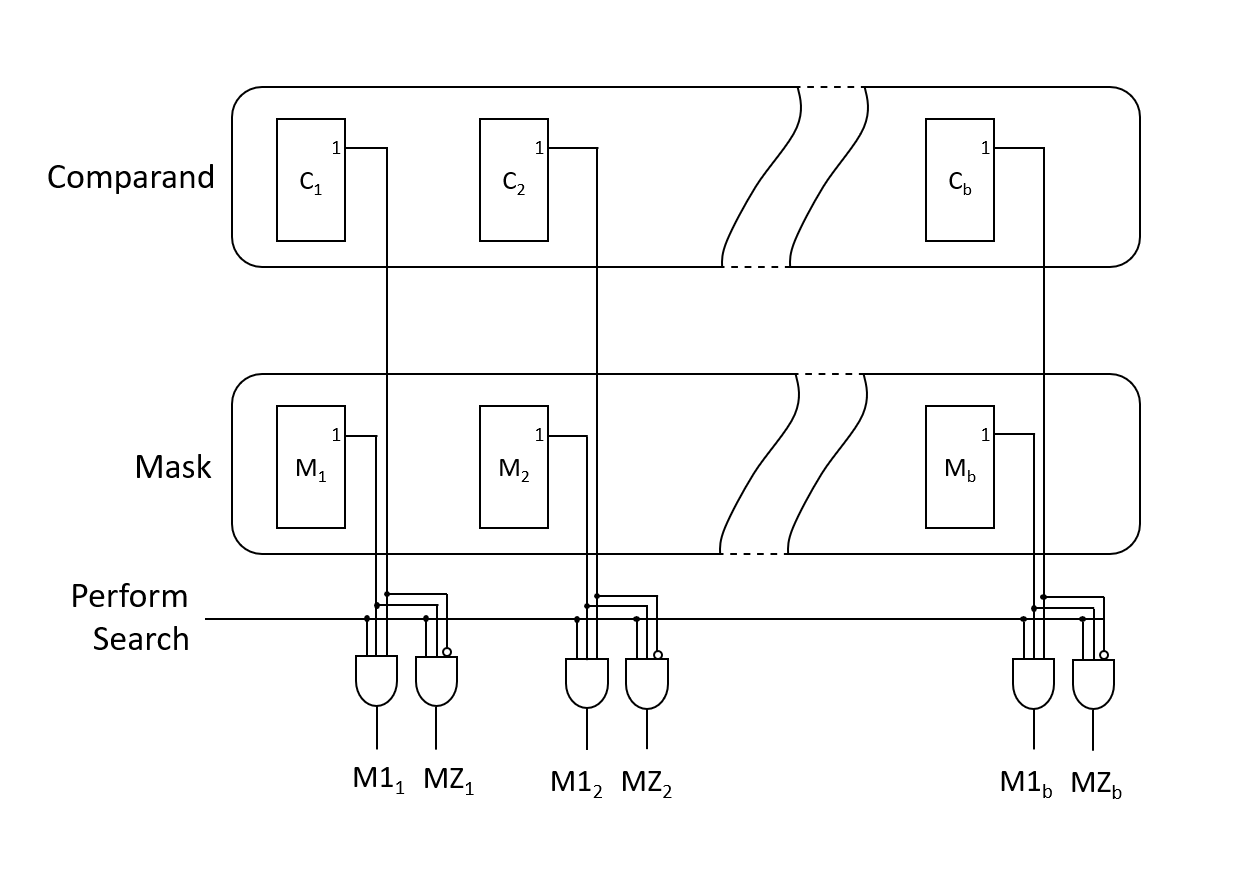
\includegraphics[width=1\columnwidth]{search_registers.png}
    \caption[Short text]{Circuitry for match lines from the search registers}
\end{figure}
\\\\
The second most complex circuitry is found in the tags.
Tags are bits for all cells, if the bit of a cell is high after a search, it means that the word in that cell was found in the search. 
In other words, after a search, the cells with high tag bits are the ones that were found. 
As all the tag bits of a CAM have to change in constant time (or in parallel), match lines from the search registers go through each cell to create mismatch lines which turn irrelevant tags off whenever the search signal is set.
The circuitry also includes logic for manually setting all bits high and selecting the first tag bit that is on.
\begin{figure}
    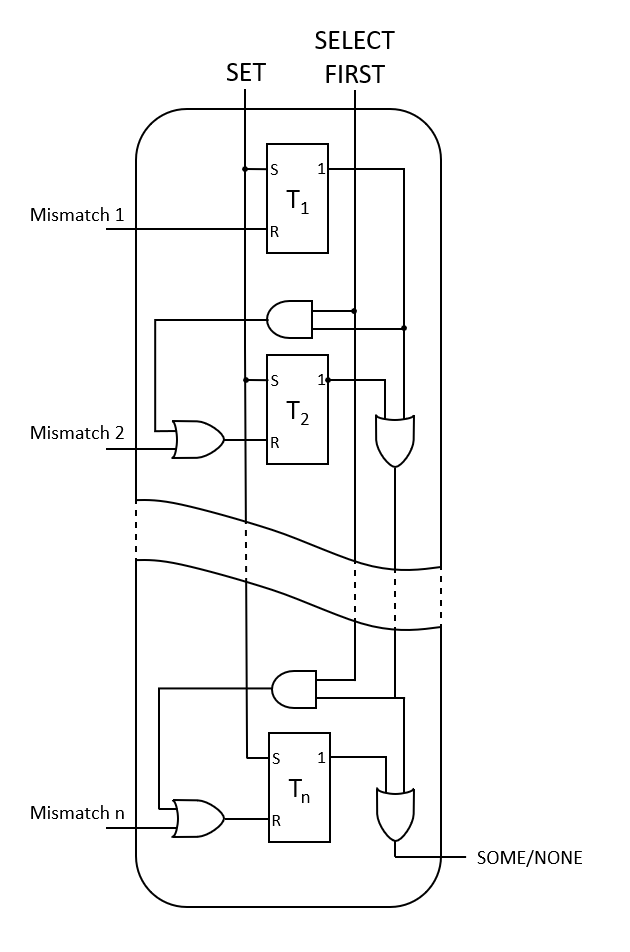
\includegraphics[width=1\columnwidth]{tag_registers.png}
    \caption[Short text]{Circuitry for tag registers}
\end{figure}
\\\\
The most complex circuitry is found in the memory cells as it encapsulates the main logic for writing, reading and searching. 
Each bit of each cell is surrounded by 2 write lines, 2 search lines and 1 read line. 
The value of each bit in each cell is changed to 0 or 1 depending on which write line is set high. 
Inversely, depending on the 2 search lines and the bit value, a mismatch line is set high or low. 
This allows the CAM to search or write in parallel. 
The output of all the read lines is the bitwise OR of all cells that have their tag bits on. 